% ==========================================
% F1 - THU LOI STATIC ROUTING TREN L10
% Nhom K = 7126
% ==========================================

\section{F1 -- Thử lỗi static routing trên liên kết L10}
\label{sec:F1}

\subsection{Mục tiêu}

Thử nghiệm F1 kiểm tra khả năng sử dụng floating static route
trên D1 khi đường chính qua C1 gặp lỗi.
Theo yêu cầu đề bài, nhóm tắt L10 ở cả hai đầu,
chạy ping liên tục từ LAN-D tới LAN-A và ghi nhận
default route mới của D1 cùng số gói bị mất.

Hai LAN được đại diện bởi Loopback1 của D1
(\texttt{10.171.126.193}, mạng LAN-D /26)
và Loopback1 của A1
(\texttt{10.171.126.1}, mạng LAN-A /26).
Liên kết thử lỗi L10 nối Fa0/0 của D1 với Fa1/0 của C1;
L11 nối D1 với B2 là đường dự phòng.

\subsection{Cách thực hiện}

\subsubsection{Kiểm tra trạng thái trước khi gây lỗi}

Trên D1, nhóm kiểm tra bảng định tuyến
và các static route đã cấu hình ở Phần A:

\begin{lstlisting}
show ip route
show running-config | include ip route
\end{lstlisting}

\partzeroimage
{images/testing/F1/D1_route_before.png}
{Bảng định tuyến và hai default route trên D1 trước khi gây lỗi L10}
{fig:F1-route-before}

Hình~\ref{fig:F1-route-before} ghi nhận default route
đang hoạt động là \texttt{0.0.0.0/0} qua C1
\texttt{10.71.26.37}, với AD 1.
Tuyến dự phòng qua B2 \texttt{10.71.26.41}
có AD 200 đã có trong cấu hình.
Các đường về LAN-D trên C1 và B2 đã được kiểm tra tại
Hình~\ref{fig:partA-c1-static}
và Hình~\ref{fig:partA-b2-static}.

\subsubsection{Chạy ping liên tục từ LAN-D tới LAN-A}

Trước khi mở phiên Telnet, nhóm tạo tài khoản cục bộ
và cấu hình các line VTY trên D1:

\partzeroimage
{images/testing/F1/D1_telnet_config.png}
{Cấu hình tài khoản cục bộ và cho phép truy cập Telnet trên D1-7126}
{fig:F1-telnet-config}

Hình~\ref{fig:F1-telnet-config} cho thấy tài khoản
\texttt{f1test} được tạo với \texttt{privilege 15}.
Nhóm chọn các line VTY từ 0 đến 4 bằng lệnh
\texttt{line vty 0 4}, dùng \texttt{login local}
để xác thực bằng tài khoản cục bộ
và \texttt{transport input telnet} để cho phép kết nối Telnet.

Để vừa duy trì ping vừa thao tác trên console D1,
nhóm sử dụng một phiên Telnet từ B2 tới địa chỉ
\texttt{10.71.26.42} của D1 trên L11.

\begin{figure}[H]
\centering
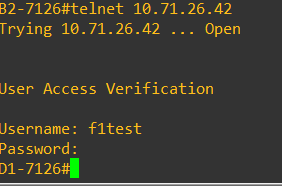
\includegraphics[width=0.38\textwidth]{images/testing/F1/B2_telnet_D1.png}
\caption{Đăng nhập D1 từ B2 qua L11 để thực hiện ping trong khi thử lỗi}
\label{fig:F1-telnet}
\end{figure}

Sau khi đăng nhập, prompt chuyển thành \texttt{D1-7126\#}.
Lệnh ping được thực thi trên D1 trong phiên này:

\begin{lstlisting}
D1-7126#ping 10.171.126.1 source Loopback1 repeat 2000 timeout 1
\end{lstlisting}

Địa chỉ nguồn là \texttt{10.171.126.193}, thuộc LAN-D.
Lệnh gửi tối đa 2000 gói ICMP Echo Request,
kích thước 100 byte, với thời gian chờ phản hồi
mỗi gói là 1 giây.
Khung hình bổ sung khi bắt đầu lượt ping có đồng hồ
hiển thị \texttt{00:01:42.897}; cửa sổ D1
đã xuất hiện một dấu \texttt{.} ở thời điểm này.

\subsubsection{Tắt L10 ở cả hai đầu}

Trong khi ping đang chạy, nhóm lần lượt tắt
cổng Fa0/0 trên D1 và Fa1/0 trên C1.
Ngay sau khi tắt phía D1, ping mất 1 gói rồi
nhận phản hồi bình thường trở lại khi phía C1 chưa bị tắt.
Sau đó, nhóm shutdown phía C1 và tiếp tục theo dõi;
không ghi nhận thêm gói mất ở bước này.
Các lệnh thực hiện như sau:

\begin{lstlisting}
! D1-7126
conf t
interface FastEthernet0/0
 shutdown
end

! C1-7126
conf t
interface FastEthernet1/0
 shutdown
end
\end{lstlisting}

Trong GNS3/Dynamips, tắt một đầu không làm
đầu bên kia tự nhận biết cổng bị down.
Vì vậy, cả hai cổng của L10 được shutdown
đúng yêu cầu F1, còn L11 được giữ hoạt động.

\partzeroimage
{images/testing/F1/D1_shutdown.png}
{Mốc đã tắt L10 phía D1: đồng hồ bản ghi hiển thị 00:01:53.497}
{fig:F1-d1-shutdown}

\partzeroimage
{images/testing/F1/both_ends_shutdown.png}
{Mốc đã tắt L10 ở cả D1 và C1: đồng hồ hiển thị 00:01:54.813}
{fig:F1-both-shutdown}

\subsection{Kết quả và giải thích}

\subsubsection{Default route mới của D1}

Sau khi kết thúc lượt ping, nhóm kiểm tra lại
bằng lệnh \texttt{show ip route} trên D1.

\partzeroimage
{images/testing/F1/D1_route_after.png}
{D1 sử dụng default route dự phòng qua B2 sau khi L10 bị tắt}
{fig:F1-route-after}

Hình~\ref{fig:F1-route-after} cho thấy
\texttt{Gateway of last resort} đã đổi sang
\texttt{10.71.26.41}. Tuyến được cài đặt là:

\begin{lstlisting}
S* 0.0.0.0/0 [200/0] via 10.71.26.41
\end{lstlisting}

Giá trị \texttt{[200/0]} xác nhận tuyến dự phòng
với AD 200 đã được sử dụng.
Mạng kết nối trực tiếp của L10
\texttt{10.71.26.36/30} không còn xuất hiện,
trong khi mạng L11 \texttt{10.71.26.40/30}
vẫn có trong bảng định tuyến.

Khi Fa0/0 trên D1 bị shutdown,
đường tới next-hop C1 qua L10 không còn hợp lệ,
nên default route chính bị loại khỏi bảng định tuyến.
Tuyến qua B2 vẫn hợp lệ và được chọn thay thế.
D1 thực hiện chuyển tuyến dựa trên trạng thái interface
và các static route đã cấu hình, không cần chạy
giao thức định tuyến động.
Khi C1 được shutdown sau đó, default route của D1
đã chuyển sang B2 nên D1 không cần đổi default route thêm lần nữa.
Điều này phù hợp với việc không mất thêm gói ở bước tắt C1.

\subsubsection{Kết quả ping giữa hai LAN}

\partzeroimage
{images/testing/F1/D1_ping_result.png}
{Kết quả ping từ LAN-D tới LAN-A trong lượt thử lỗi F1}
{fig:F1-ping-result}

Hình~\ref{fig:F1-ping-result} ghi nhận
\texttt{1997/2000} gói thành công,
tương ứng \textbf{3 gói bị mất} trong toàn bộ lượt ping.
Tỷ lệ tính từ số gói là \textbf{99,85\%};
output IOS hiển thị phần trăm nguyên là \texttt{99 percent}.
RTT min/avg/max lần lượt là \textbf{120/152/192 ms}.

Đối chiếu output với quan sát trong quá trình thao tác,
nhóm ghi nhận:
\begin{itemize}
    \item Trước khi gây lỗi: mất 2 gói ở đầu lượt ping.
    \item Khi shutdown D1, trong lúc C1 chưa shutdown:
    mất thêm 1 gói, sau đó ping bình thường trở lại.
    \item Khi shutdown C1 sau đó: không mất thêm gói.
\end{itemize}

Như vậy, số gói mất gắn với thử lỗi L10 là \textbf{1 gói};
tổng \textbf{3 gói} trong thống kê cuối còn bao gồm
2 gói mất trước khi gây lỗi.
Kết nối giữa hai LAN đã phục hồi trước bước tắt C1.

\begin{table}[H]
\centering
\caption{Kết quả thử lỗi static routing trong F1}
\label{tab:F1-results}
\small
\renewcommand{\arraystretch}{1.3}
\begin{tabularx}{\textwidth}{X l}
\toprule
\textbf{Nội dung} & \textbf{Kết quả} \\
\midrule
Default route trước lỗi & Qua C1: \texttt{10.71.26.37}, AD 1 \\
Default route sau lỗi & Qua B2: \texttt{10.71.26.41}, AD 200 \\
Gói ping thành công & 1997/2000 \\
Gói mất trong toàn lượt ping & 3 \\
Gói mất trước khi gây lỗi & 2 \\
Gói mất sau shutdown D1 & 1, rồi ping bình thường trở lại \\
Gói mất thêm sau shutdown C1 & 0 \\
Tỷ lệ thành công tính từ số gói & 99,85\% \\
RTT min/avg/max & 120/152/192 ms \\
Mốc khung hình bắt đầu ping & 00:01:42.897 \\
Ping bình thường trở lại & Trước khi shutdown C1 \\
\bottomrule
\end{tabularx}
\end{table}

\subsubsection{Đối chiếu các mốc thời gian}

Khung hình bắt đầu ping hiển thị \texttt{00:01:42.897};
các khung hình đã tắt phía D1 và tắt cả hai đầu
lần lượt hiển thị \texttt{00:01:53.497}
và \texttt{00:01:54.813}.
Như vậy, hai thao tác được ghi nhận sau mốc bắt đầu ping
lần lượt \textbf{10,600 giây} và \textbf{11,916 giây},
cách nhau \textbf{1,316 giây}.
Các khoảng này mô tả trình tự thử nghiệm.
Theo quan sát, ping chỉ mất 1 gói sau khi tắt D1
và đã bình thường trở lại trước khi tắt C1.
Với timeout 1 giây, kết quả thể hiện một lần thăm dò
không nhận phản hồi trong thời hạn chờ.

\subsection{Khôi phục sau thử nghiệm}

Để đưa mô hình về trạng thái ban đầu,
bật lại cả hai cổng của L10:

\begin{lstlisting}
! D1-7126
conf t
interface FastEthernet0/0
 no shutdown
end

! C1-7126
conf t
interface FastEthernet1/0
 no shutdown
end
\end{lstlisting}

Sau đó kiểm tra \texttt{show ip route} trên D1,
xác nhận default route qua C1 với AD 1 được ưu tiên trở lại,
và chờ ping giữa hai LAN ổn định trước khi chuyển sang F2.

\newpage
